\section{Experiments}%
\label{sec:experiments}

Here, we provide additional details about our framework, benchmark it against state-of-the-art rigid and dynamic reconstruction methods, and ablate key design choices.

\subsection{Implementation Details}

We focused on four model variants: $200$M, $500$M, $1$B, and $10$B parameters, with $12/12/24/16$ alternating-attention blocks and hidden sizes $384/768/1024/4096$, respectively.
The vision transformer is initialized from DINOv3~\cite{simeoni25dinov3} and is not frozen during training.
Each block contains one global attention (or register attention) layer and one frame-wise attention layer.
Optimization uses AdamW for $240$K iterations, with $160$K supervised, $50$K self-supervised, and a final $30$K supervised stage.
The learning rate follows a linear warm-up over $5\%$ of training and cosine decay for the remaining $95\%$, with a peak value of $2\times10^{-4}$ for supervised training and $1\times10^{-4}$ for self-supervised training.
For each batch, the number of frames is drawn uniformly from $[1,24]$.
We augment images by randomly varying the aspect ratio within \([0.33,1.33]\), keeping the image area approximately $512 \times 512$ pixels, and applying color jittering, grayscale conversion, and random patch masking.
Training used $128$ $96$GB H100 GPUs, bfloat16 mixed precision, gradient checkpointing, and FSDP.

\subsection{Benchmarking}%
\label{sec:benchmarking}

\begin{figure*}
\centering
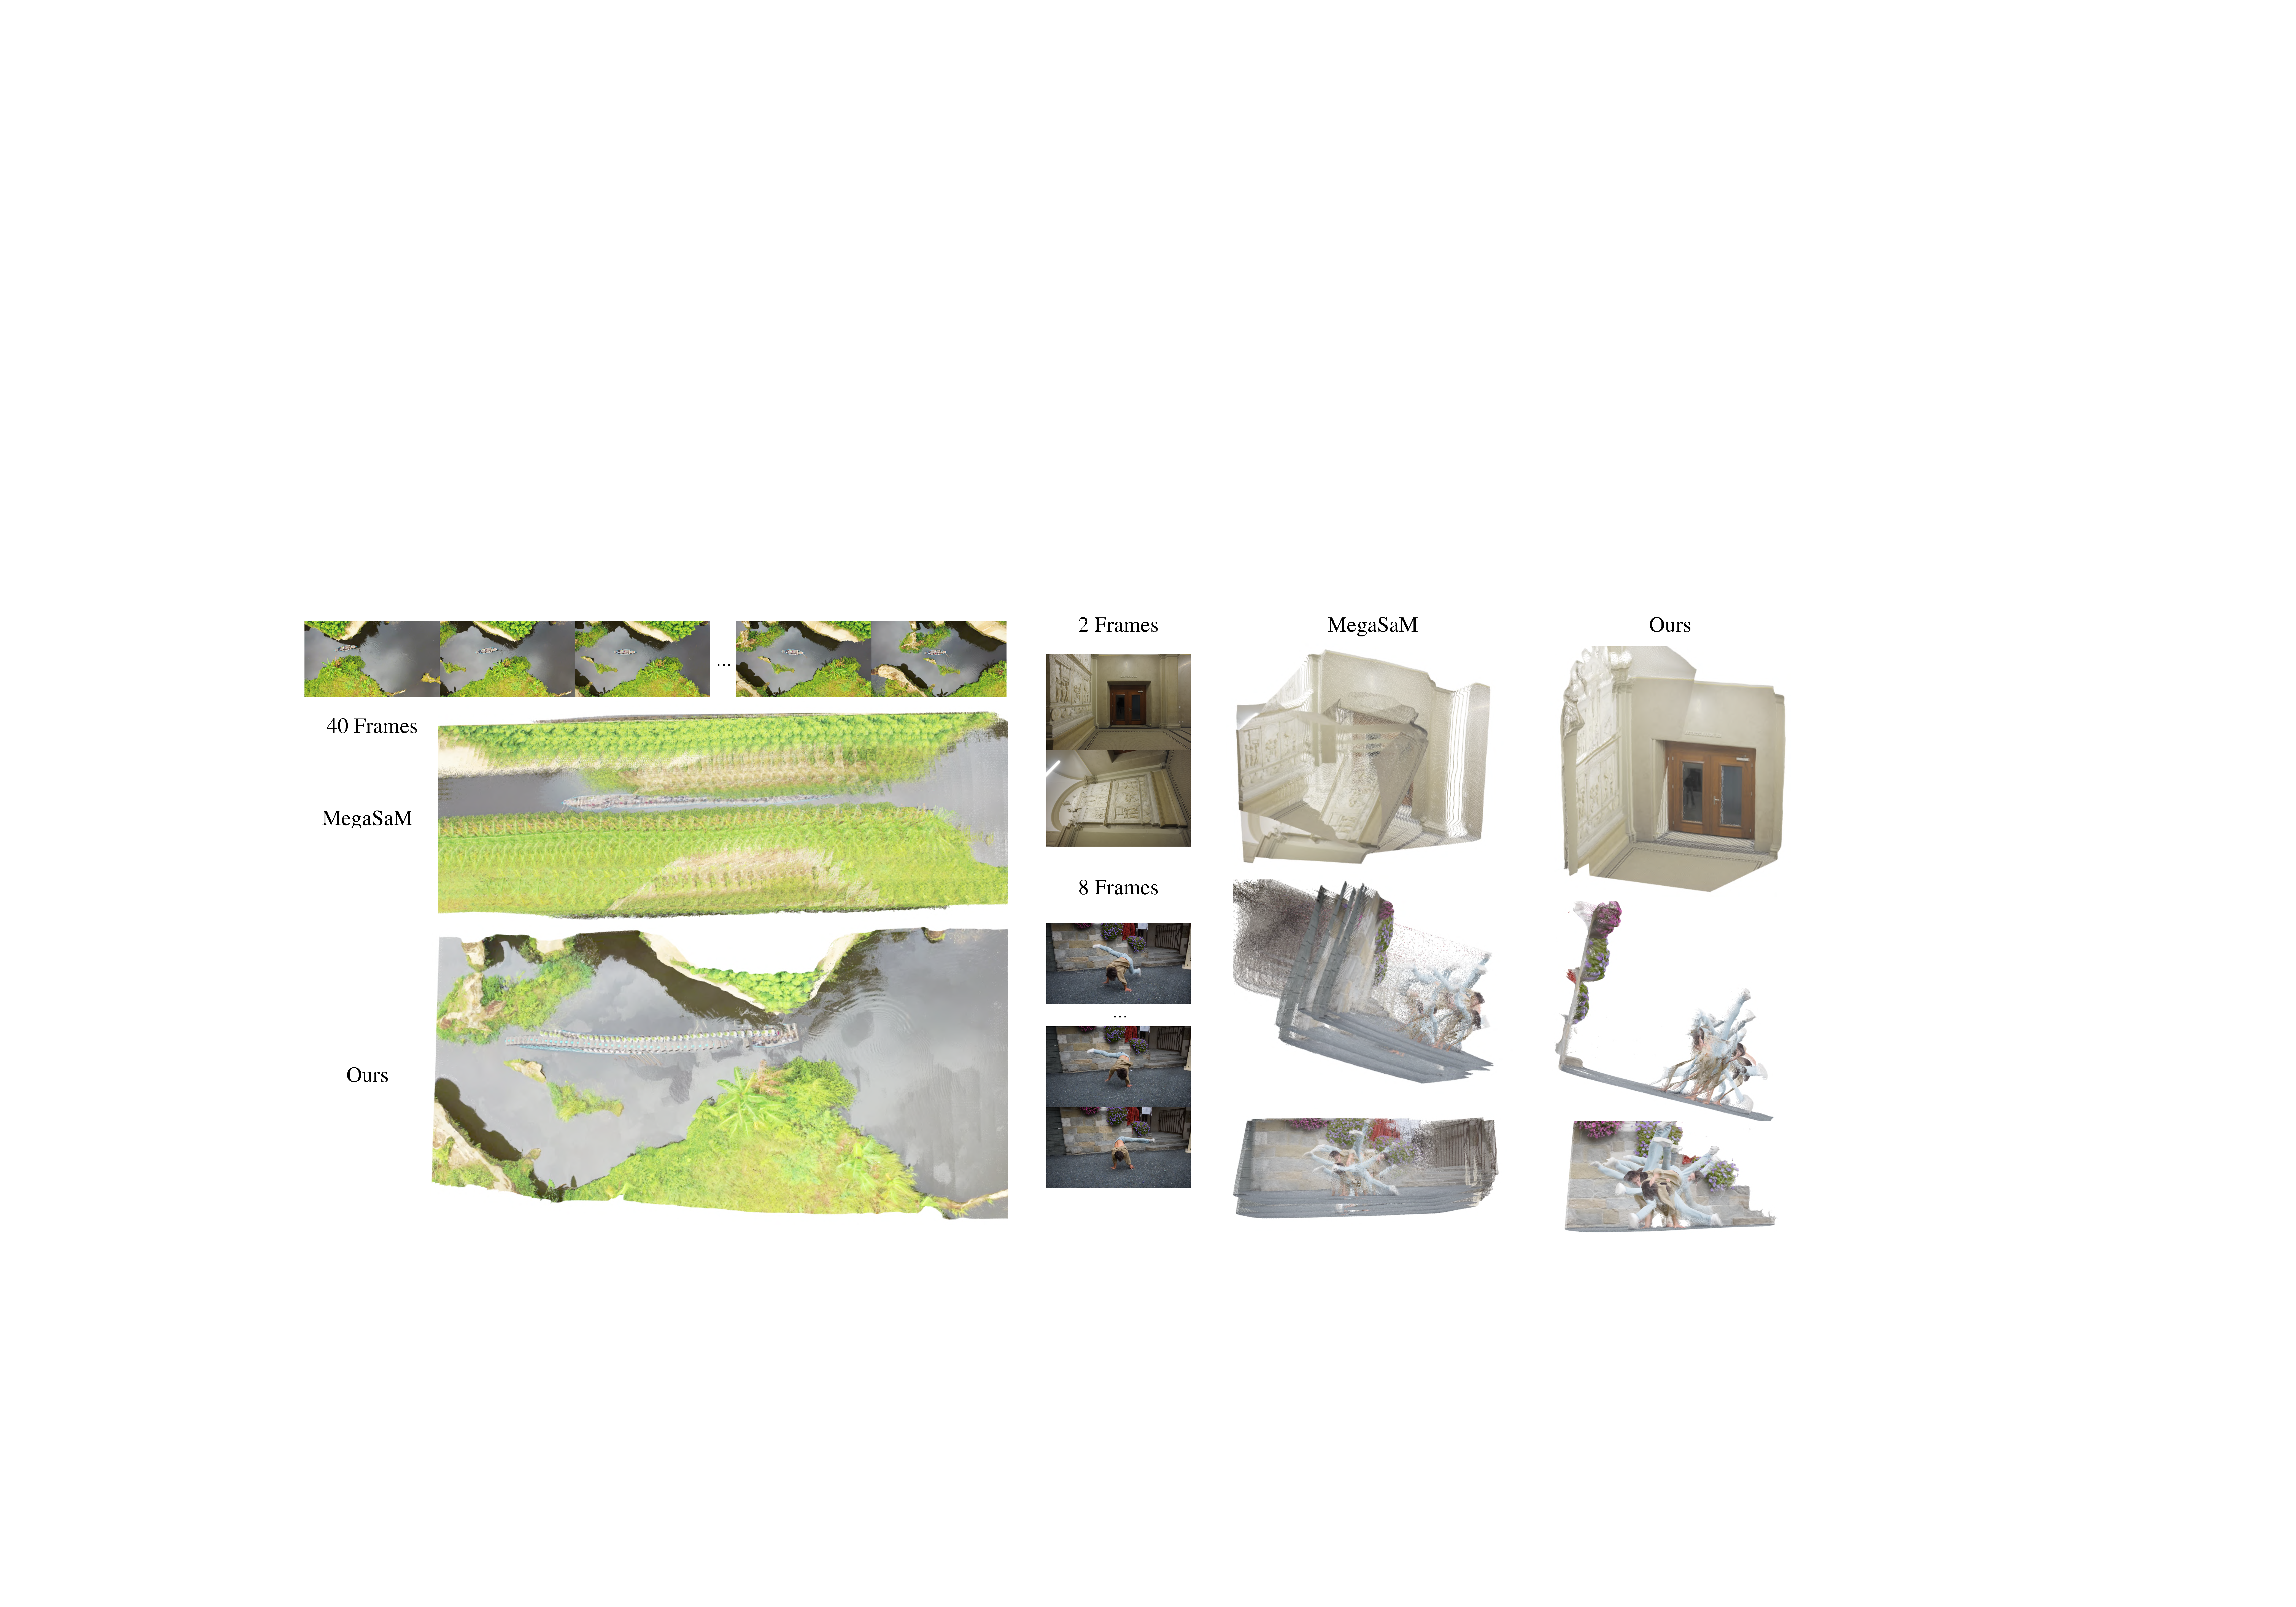
\includegraphics[width=1.0\textwidth]{figures/qual_supp_v10.pdf}
\caption{\textbf{Qualitative Comparison to MegaSaM.} 
MegaSaM often suffers from geometric inconsistencies. 
In contrast, our method produces globally consistent reconstructions across sparse, dynamic, and aerial scenarios. 
This is especially evident in the aerial scene in the left column, where MegaSaM exhibits severe geometric drift and texture smearing, resulting in repeated patterns and a distorted global layout.
Note that the second frame in the top right example is not upright, which makes this case particularly challenging. 
}%
\label{fig:qual_supp}
\end{figure*}

\paragraph{Quantitative Comparison.}



We compare \method with recent approaches:
(i) feed-forward reconstruction models and (ii) optimization-based dynamic reconstruction methods.
We evaluate on three static datasets (7 Scenes~\cite{shotton13scene}, NRGBD~\cite{azinovic22neural}, and ETH3D~\cite{schops17a-multi-view}) and three dynamic datasets (DyCheck~\cite{gao22monocular}, Sintel~\cite{butler12a-naturalistic}, and TUM-Dynamic~\cite{sturm12a-benchmark}).
For each scene or sequence, we randomly sample $10$ frames.
We use the original released models for all methods.
For DA3, we use its largest variant, Giant (1B parameters).

Following~\cite{wang25vggt}, we report the standard AUC for camera pose estimation (higher is better), computed as the area under the curve of the fraction of image pairs whose relative rotation and translation errors fall below an angular threshold (\eg, $3^\circ$, $30^\circ$).
As shown in \cref{tab:camera}, feed-forward models generally exhibit strong performance on static benchmarks and at more relaxed thresholds, while optimization-based, dynamic-aware MegaSaM is more competitive on challenging dynamic sequences such as Sintel but degrades on wide-baseline or low-texture scenes.
In contrast, our models consistently outperform all baselines across both static and dynamic datasets and at both strict and relaxed thresholds.

We also evaluate the accuracy of the predicted depths using absolute relative error (AbsRel; lower is better) and $\delta_{1.25}$ (higher is better), which measures the percentage of pixels for which the ratio of the predicted depth to the ground-truth depth is within a specified threshold.
As shown in \cref{tab:depth}, our models outperform the baselines in the static benchmarks, further lowering AbsRel on datasets where existing methods perform strongly, such as ETH3D, and even more so in dynamic scenes, where they reduce depth errors and increase $\delta_{1.25}$ (\eg, on Sintel, improving $\delta_{1.25}$ from $86.1$ to $93.5$ and AbsRel from $0.118$ to $0.081$).

The larger 10B variant consistently outperforms the 1B model, indicating that scaling up the reconstruction model directly benefits both camera and depth accuracy.

\paragraph{Qualitative Results.}

\Cref{fig:qual} illustrates our results on static and dynamic scenes, including traffic, human motion, natural landscapes, and underwater environments.

\begin{figure*}
\centering
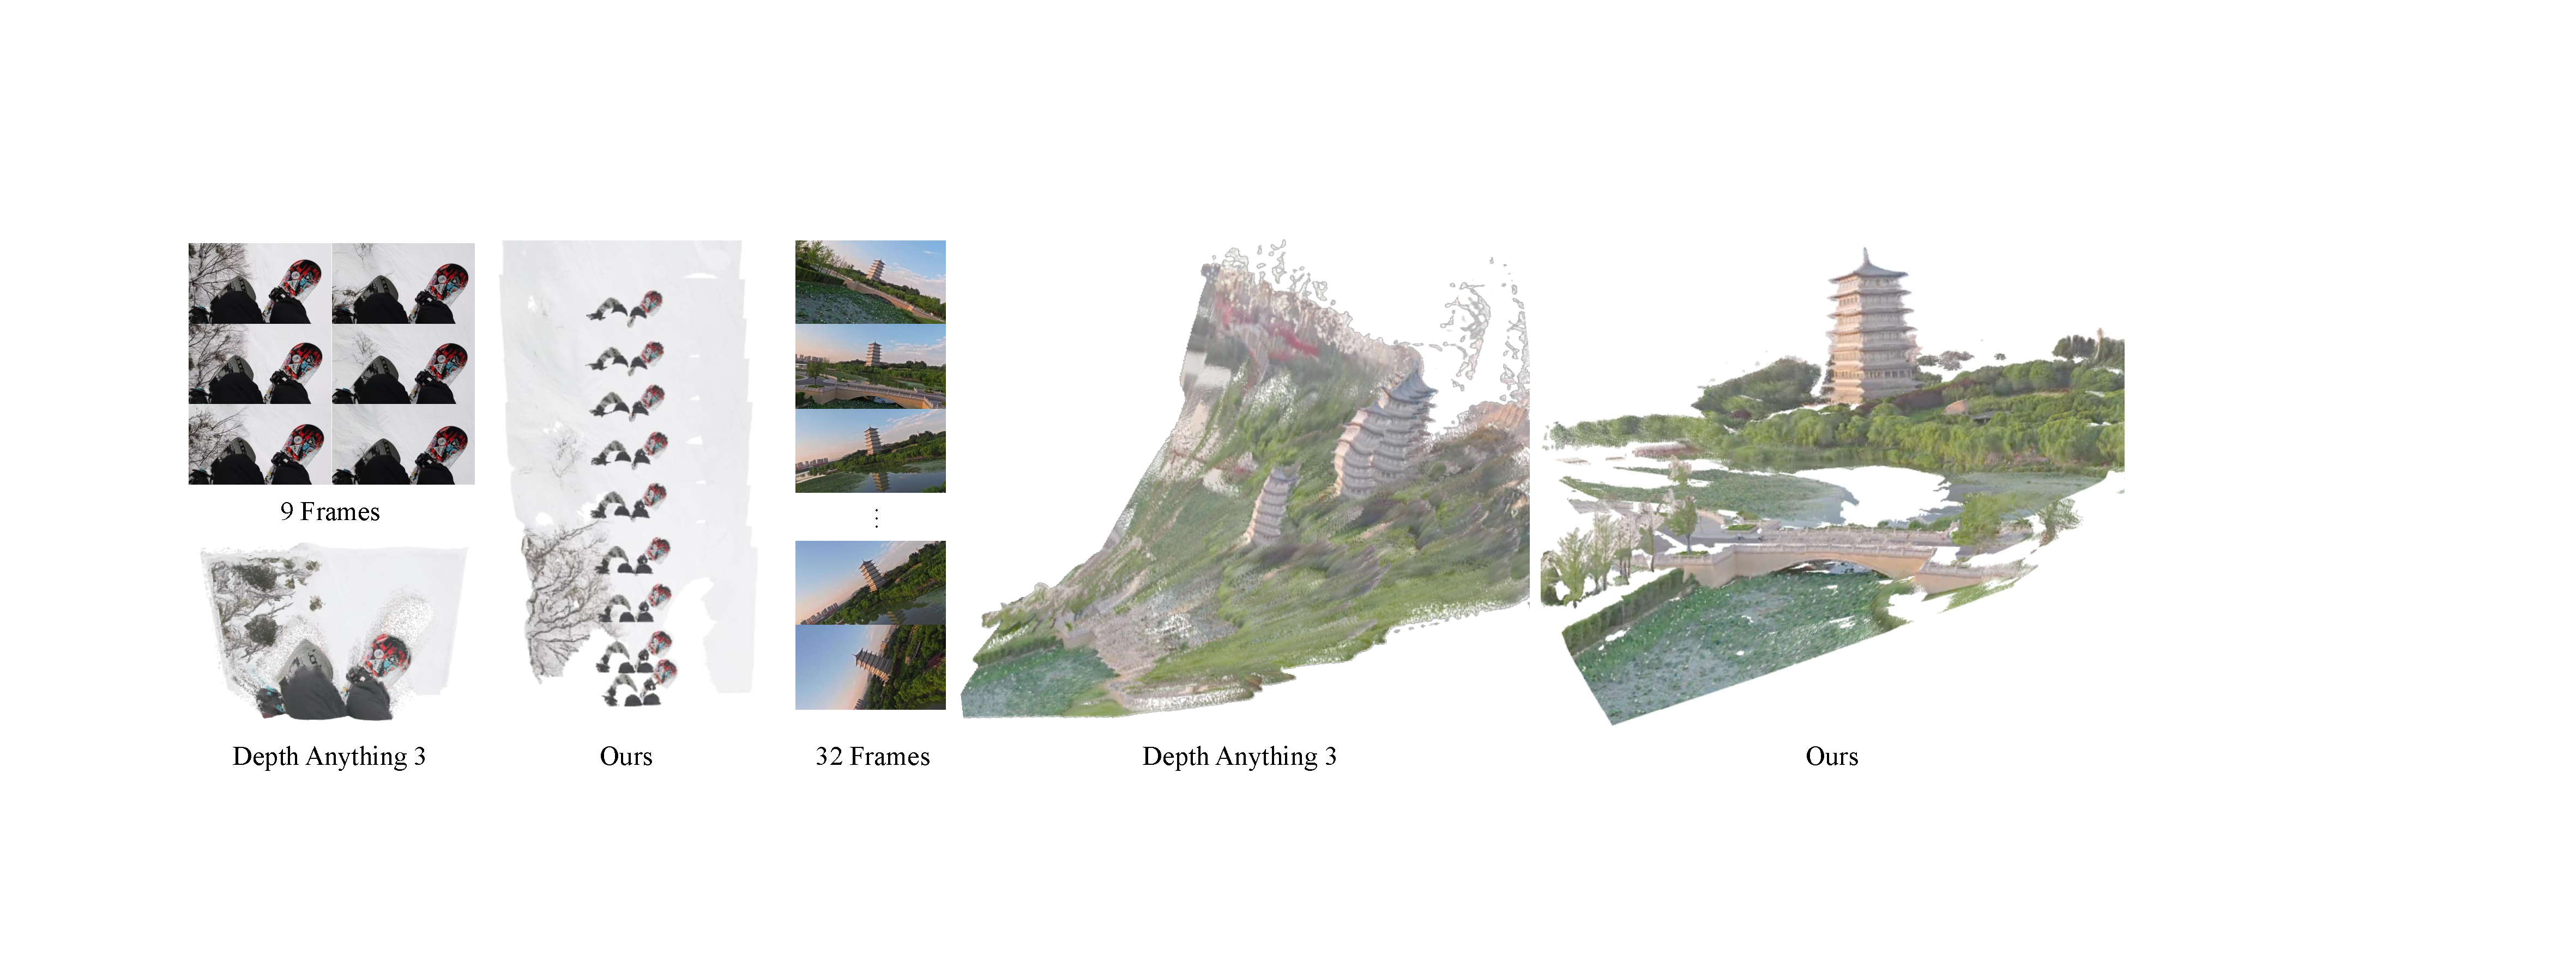
\includegraphics[width=\textwidth]{figures/qual_comp_to_da3.pdf}
\caption{\textbf{Qualitative Comparison to Depth Anything 3.}
\emph{Left:} a snow lift sequence over a snow-covered field, where the repetitive terrain misleads DA3 into estimating little to no camera motion.
Our method recovers the correct camera trajectory.
\emph{Right:} a drone sequence in which the camera rolls while flying toward a tower.
Under this strong viewpoint change, DA3 produces severe ghosting and duplicated tower structures, whereas our reconstruction remains globally consistent.}%
\label{fig:qual_da3}
\end{figure*}








\begin{figure}[htbp]
\centering
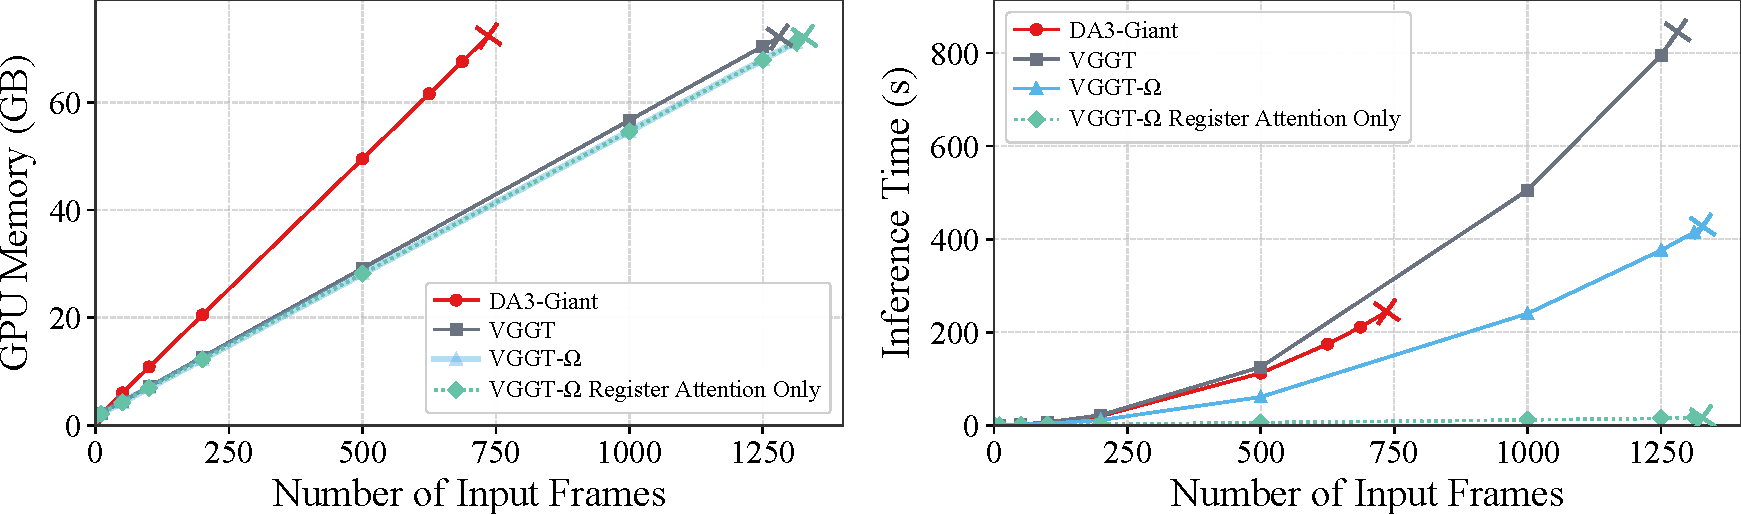
\includegraphics[width=\linewidth]{figures/mem_speed_v2_vector.pdf}
\caption{\textbf{Memory and Speed Comparison.}
We compare the inference memory usage and runtime of VGGT, DA3, and \method on an 80GB A100 GPU with flash attention v2 enabled.
For VGGT, we first address an implementation detail which improves its efficiency (see text).
Cross markers indicate the first setting at which each method runs out of memory.
}%
\label{fig:mem_speed}
\end{figure}



We further compare \method with DA3 and MegaSaM on challenging cases in \cref{fig:qual_da3,fig:qual_supp}.
In \cref{fig:qual_da3}, DA3 struggles with repeated textures, estimating little to no camera motion in the snow lift sequence, and with strong camera roll, reconstructing the tower several times in the drone sequence.
MegaSaM can also break down in sparse indoor scenes with substantial camera roll (top right) or textureless walls (bottom right), producing disjoint structures or misaligned planes, while certain aerial sequences (left) also challenge its pose estimation.
In contrast, \method's reconstructions are globally consistent, likely due to the strength of the geometric priors learned from diverse data.


\paragraph{Inference Memory and Speed.}



We now compare the \emph{inference} memory and speed of \method with VGGT and DA3\@ (note that this is quite different from the training efficiency discussed in \cref{sec:architecture}).

For these comparisons, we first correct the original VGGT implementation.
That model caches intermediate tensors from all $24$ layers during inference.
Although these cached tensors are useful during training, the prediction heads only require intermediate features from four layers at test time.
We thus avoid caching unnecessary information, which substantially reduces inference memory usage.

With this correction in place, we compare VGGT, DA3, and \method in \cref{fig:mem_speed}. 
For a fair comparison, all measurements are conducted on a single 80GB A100 GPU using PyTorch \textit{scaled\_dot\_product\_attention}, with a flash attention v2 backend. 
We use similar input resolutions matched to each model's patch size: $518 \times 336$ for VGGT and DA3 with $14$-pixel patches, and $512 \times 336$ for \method with $16$-pixel patches.
We increase the number of input frames until each method runs out of memory, as indicated by the cross markers in \cref{fig:mem_speed}.

As for memory efficiency, VGGT (with the correction) and \method are similar, and can process more than $1,\!000$ frames on a single A100 GPU\@.
As for speed, \method is faster, primarily due to using DINOv3, with a patch size of $16$, instead of DINOv2, with a patch size $14$, which reduces the number of image tokens by about $25\%$.
In addition, \method replaces $25\%$ of the global attention layers with register attention by default, reducing FLOPs and yielding a $20$--$25\%$ speedup.
Overall, VGGT and \method scale more favorably than DA3 in both memory and runtime, \eg, DA3 runs out of memory at around $750$ frames in our testing, whereas VGGT and \method can handle around $1250$ frames.
An even more aggressive variant of \method that replaces all global attention layers with register attention can further improve speed, reducing the runtime on $1000$ frames from $240.2$ seconds to $11.7$ seconds, albeit at the cost of lower reconstruction accuracy (\cref{sec:discussion}).


While perhaps surprising, we stress that, during inference, the main benefit of removing global attention is speed, not memory.
As shown in \cref{fig:mem_speed}, replacing all global attention layers with register attention produces a large speedup, while peak inference memory remains almost unchanged. 
The speedup is because register attention avoids computing interactions between all pairs of image tokens, unlike global attention.
However, with PyTorch \textit{scaled\_dot\_product\_attention} using flash attention v2, the full attention matrix is not explicitly materialized in memory. 
Instead, the kernel computes attention in a tiled streaming manner, updates the softmax normalization online, and directly accumulates the output.
Peak memory is instead dominated by tensors whose size is proportional to the number of frames and image tokens, such as frame-attention activations or feed-forward intermediates.
This explains why memory grows approximately linearly with the number of frames in \cref{fig:mem_speed}. 



\subsection{Ablation Studies}

Unless otherwise specified, ablations use the 1B model variant trained on $2$M sequences with $64$ GPUs for $150$k supervised steps.
To jointly assess camera and depth accuracy, we unproject depth maps into 3D using the cameras and compute the $\ell_2$ distance between the predicted and ground-truth points, which we call \emph{point error}.
We use point error rather than Chamfer distance because nearest-neighbor matching over unordered point sets can be dominated by large surface regions such as walls and floors.
All the models are trained on approximately the same number of tokens.

\paragraph{Model and data size.}

We observe that scaling either the model or the data consistently improves performance, as shown in \cref{fig:scale}.
Increasing the number of training sequences in $10\times$ steps yields a monotonic drop in point error, from $0.275$ to $0.073$.
Overall, the shape of both curves suggests that power laws might characterize scaling in this class of models.

\paragraph{Register attention.}

A variant that uses only global attention layers achieves a point error of $0.071$.
Replacing 25\% of the global attention layers with register attention yields performance nearly identical to the original ($0.073$).

\paragraph{Multi-task learning.}

Removing the point and matching losses increases the point error from $0.073$ to $0.078$.
For reference, adopting VGGT's original multi-head, multi-task setup achieves $0.070$ but requires multiple dense heads, making scaling difficult.

\paragraph{Self-supervised training.}

Replacing $10\%$ of training steps from supervised training with self-supervised training slightly reduces point error from $0.073$ to $0.070$.
This performance gain stems from training on unlabeled data, which is more diverse.
We also observe improved out-of-distribution generalization.

\paragraph{Annotation quality.}

To validate the quality of the pseudo ground truth produced by our annotation pipeline, we compare it against MegaSaM~\cite{li25megasam:} on Sintel, which provides synthetic camera and depth ground truth.
For a fair comparison, we evaluate only the sequences and pixels that satisfy both our filtering criteria and MegaSaM's validation, excluding $8/23$ sequences and all dynamic regions.
Under this protocol, our pipeline achieves $96.4\%$ AUC@$30^\circ$ for camera pose and $99.3\%$ $\delta_{1.25}$ for depth, compared with $62.1\%$ and $77.2\%$ for MegaSaM, respectively, confirming the high quality of the resulting annotations.
Our goal in pseudo-label generation is not to maximize yield, but to retain only sequences and pixels that are very likely to be correct, as we find that a smaller set of highly accurate pseudo ground truth is more beneficial in practice than a larger but noisier collection.
Hence, the annotation pipeline is intentionally conservative: if a sequence is even mildly ambiguous, or if a pixel cannot be validated reliably, we prefer to discard it rather than risk injecting noisy supervision.

\subsection{Applications of Registers}%
\label{sec:applications}

\paragraph{Robotics.} Recent work has explored the use of reconstruction models to improve spatial understanding in VLA systems~\cite{li25spatial, abouzeid25geoaware-vla:}.
We evaluate whether \method can be a plug-and-play geometric encoder for VLA\@.
Given the input images, we extract registers (scene tokens) from \method and concatenate them with the original OpenVLA-OFT input tokens~\cite{kim25fine-tuning}.
We then train OpenVLA-OFT using its standard protocol, while keeping \method fixed throughout.
As shown in \cref{tab:vla}, the geometry-aware registers consistently improve performance across all LIBERO tasks~\cite{liu23libero:}.

\begin{table}[htbp]
\centering
\caption{\textbf{Performance on the LIBERO benchmark.}
We freeze our pretrained model, feed the scene tokens as additional input to OpenVLA-OFT, and report the success rate (SR) (higher is better).
The clear gains validate the effectiveness of our scene tokens in aggregating spatial information.
}%
\label{tab:vla}
\scriptsize
\renewcommand{\tabcolsep}{4pt}
\begin{tabular}{cccccc}
\toprule
\multicolumn{1}{c}{Method}
& \begin{tabular}[c]{@{}c@{}}Spatial\\ SR (\%)\end{tabular}
& \begin{tabular}[c]{@{}c@{}}Object\\ SR (\%)\end{tabular}
& \begin{tabular}[c]{@{}c@{}}Goal\\ SR (\%)\end{tabular}
& \begin{tabular}[c]{@{}c@{}}Long\\ SR (\%)\end{tabular}
& \begin{tabular}[c]{@{}c@{}}Average\\ SR (\%)\end{tabular}
\\ \midrule
Diffusion Policy & 78.3 & 92.5 & 68.3 & 50.5 & 72.4 \\
TraceVLA         & 84.6 & 85.2 & 75.1 & 54.1 & 74.8 \\
Octo             & 78.9 & 85.7 & 84.6 & 51.1 & 75.1 \\
OpenVLA          & 84.7 & 88.4 & 79.2 & 53.7 & 76.5 \\
Dita             & 84.2 & 96.3 & 85.4 & 63.8 & 82.4 \\
CoT-VLA          & 87.5 & 91.6 & 87.6 & 69.0 & 83.9 \\
$\pi_0$-FAST     & 96.4 & 96.8 & 88.6 & 60.2 & 85.5 \\
$\pi_0$          & 96.8 & 98.8 & 95.8 & 85.2 & 94.2 \\
UniVLA           & 96.5 & 96.8 & 95.6 & 92.0 & 95.2 \\
OpenVLA-OFT      & 97.6 & 98.4 & 97.9 & 94.5 & 97.1 \\
\midrule
\begin{tabular}[c]{@{}c@{}}OpenVLA-OFT\\ + Our Frozen Scene Tokens\end{tabular} & \textbf{99.3} & \textbf{99.2} & \textbf{99.0} & \textbf{96.7} & \textbf{98.5} \\
\bottomrule
\end{tabular}
\end{table}





\paragraph{Language Alignment.}

To further verify whether the registers contain high-level information, we investigate whether they can be aligned to natural language.
The procedure, illustrated in \cref{fig:text_alignment}, follows the spirit of CLIP-style contrastive alignment~\cite{radford21learning, zhai23sigmoid}.
However, to keep it as simple as possible, we use a well-trained \method, fix the language encoder and only fine-tune our model.

\begin{figure}
\centering
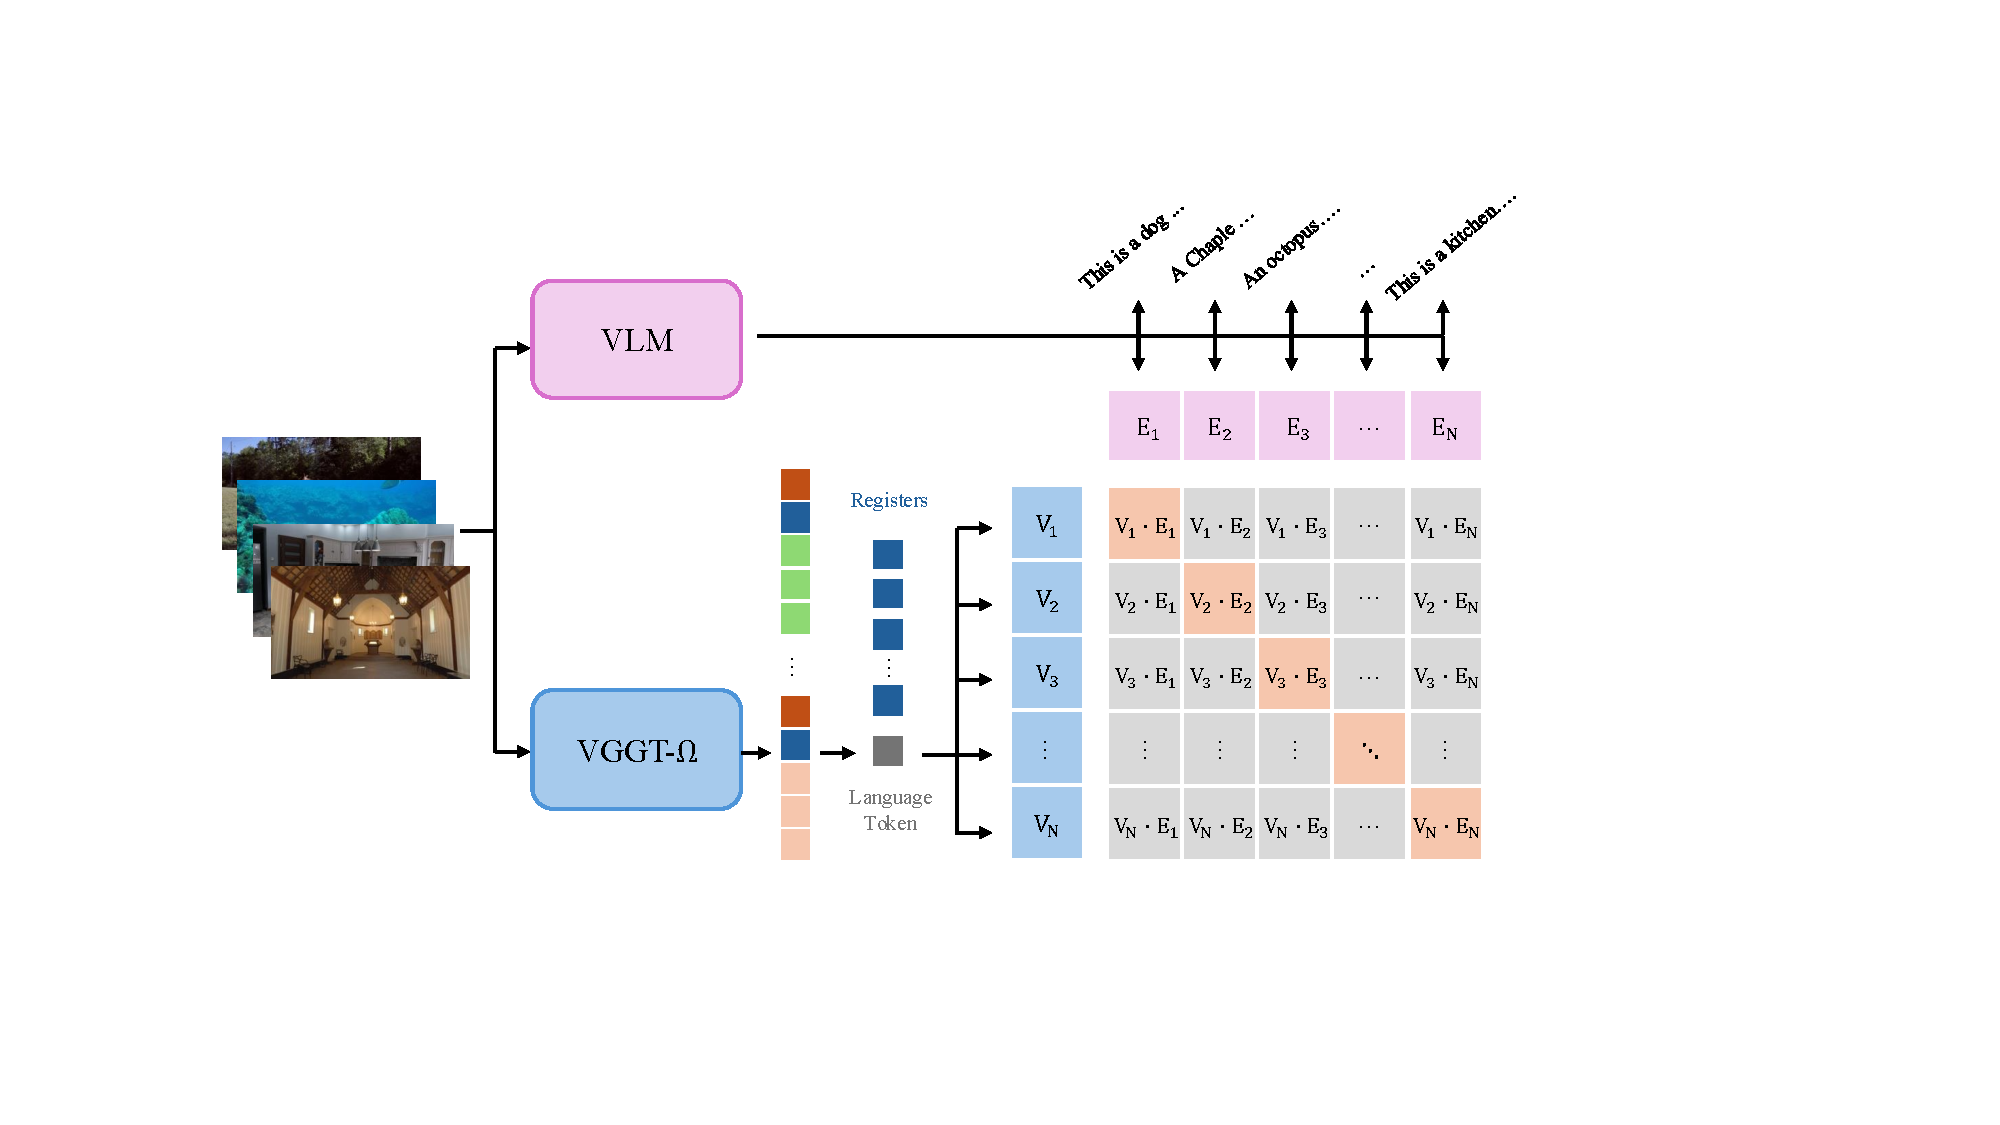
\includegraphics[width=0.95\linewidth]{figures/text_alignment.pdf}
\caption{\textbf{Language Alignment.} 
We conduct language alignment to verify whether the registers contain high-level information. 
For each sequence, a VLM describes the scene content, coarse layout, and appearance, and the generated text tokens are mean-pooled to form the language embedding. 
On the \method side, a small self-attention stack takes the registers and a learnable language token as input, and the output language token is projected to form the register-derived embedding. 
The two embeddings are optimized with a symmetric InfoNCE loss over all sequence-description pairs in the global batch.
}%
\label{fig:text_alignment}
\end{figure}



In detail, we use a VLM and \method to separately extract a global descriptor for a given image sequence and then align the two.
To extract this global descriptor, the VLM observes all input views and is prompted to describe the scene content, coarse layout, and appearance as a single coherent scene.
Then, the hidden states of the text tokens generated by the VLM are mean-pooled and $\ell_2$-normalized.
To obtain a global descriptor from \method, a small self-attention stack takes the registers and a new learnable language token (randomly initialized) as input.
The output language token is projected and $\ell_2$-normalized to produce the register-derived embedding from \method.

It is worth noting that the language token we introduced never directly observes image patch tokens, as it can only read out the registers.
Thus, a successful alignment indicates that the registers themselves carry scene-level information that can be matched to language.

We maximize the cosine similarity of the matched register-derived embeddings and VLM language embeddings while minimizing the similarity of mismatched pairs with a symmetric InfoNCE loss.
We fine-tune the models on the same image sequences as in the main reconstruction training.
As in distributed CLIP training, embeddings are gathered across GPUs so that the global batch provides in-batch negatives.
The VLM is frozen, and \method is fine-tuned end-to-end with a constant learning rate of $1\times10^{-5}$, rather than kept fixed as in the robotics experiment.

After only 10K iterations with a small learning rate, the model already transfers well to language retrieval.
For evaluation, we construct a benchmark of 100 manually curated internet videos spanning a diverse set of scenarios, including cooking, praying, car racing, and more.

Given the register-derived embedding of the aligned \method, we retrieve the paired language embedding for each candidate video using cosine similarity and report top-$K$ accuracy.
Using the VLM embedding employed during alignment, the model achieves $76.8\%$ top-1 accuracy and $97.0\%$ top-3 accuracy.
That is, the correct language description ranks among the top three candidates for almost all videos.
To test whether this alignment transfers beyond the exact training target, we replace the VLM embedding with a text-only LLM embedding, without any additional training.
Specifically, we prompt the VLM to generate a video description and feed only this description to the Qwen3 LLM~\cite{yang25qwen3}.
The model still obtains $47.5\%$ top-1 accuracy and $77.8\%$ top-3 accuracy in this zero-shot transfer setting.

Overall, these results show that the registers carry high-level information, likely quite semantic, that can be aligned with language space.
At the same time, there is no degradation on the geometric tasks after alignment fine-tuning.
The example text description and the prompt are provided in the supplementary materials.
This may indicate that representations learned by a strong geometry model can align naturally with those of other modalities, such as language.
This observation is consistent with the platonic representation hypothesis~\cite{huh24position:,han25learning}, which suggests that sufficiently capable models trained on different modalities tend to converge toward a shared representation space.

\paragraph{General Applications.}

Registers provide a general mechanism for extracting both sequence-level and frame-level representations from the model.
This design naturally extends to additional prediction tasks by introducing task-specific learnable tokens.
For sequence-level predictions, a learnable token can be concatenated to the register tokens and decoded into the desired output, similar to the language token discussed above.
For frame-level predictions, the same token can be replicated across frames, concatenated with the corresponding registers, and used to produce per-frame estimates.
We have conducted preliminary experiments on several such tasks, including metric scale estimation, gravity direction estimation, and human presence detection, and observed promising results.
We leave the exploration of these possibilities to the community.
From this perspective, a camera token can also be viewed as a register-like learnable token, with the main distinction that it is trained under direct camera supervision.












